\documentclass[12pt]{article}
\usepackage{hyperref,a4wide,color,boxedminipage,Sweave}
\usepackage[utf8]{inputenc}

%\VignetteIndexEntry{Tests in mixed effects models}
%\VignettePackage{doBy}

\special{html:
  <link title="main" media="all" rel="stylesheet" href="../../../shdcss.css"
 type="text/css" />
}
\title{Tests in mixed effects models -- some facilities in the
  \texttt{doBy} package}
\author{S{\o}ren H{\o}jsgaard and Ulrich Halekoh}
\begin{document}
\maketitle
\tableofcontents


\setkeys{Gin}{height=3in}
\renewenvironment{Schunk}{\begin{center}
    \scriptsize
    \begin{boxedminipage}{1.0\textwidth}}{
    \end{boxedminipage}\end{center}}


\def\proglang#1{{#1}}
\def\pkg#1{{#1}}
\def\doby{\pkg{doBy}}
\def\lme{\pkg{lme4}}
\def\code#1{\texttt{#1}}
\def\shd#1{\footnote{SHD: #1}}
\def\summaryby{\code{summaryBy}}
\def\R{\proglang{R}}


\parindent0pt\parskip5pt




\section{Introduction}
\label{sec:introduction}

The \doby\ package provides some facilities for improved tests for
model reductions in linear mixed models (when these are fitted with
the \code{lmer()} function in the \lme\ package. Currently, model
comparison in the \lme\ implementation is based on the large sample
$\chi^2$ approximation of the likelihood ratio statistic (LRT).

We have implemented the following alternatives:

\begin{itemize}
\item
One approach is based on constructing an "F--like" statistic and then
estimating the denominator degrees of freedom using the Kenward--Roger method.

\item The other approach is based on estimating the reference
  distribution in different ways using parametric bootstrap methods.

\end{itemize}

\subsection{Motivation: Sugar beets - A split--plot experiment}
\label{sec:xxx}


  Dependence of yield [kg] and sugar percentage of sugar beets on
  harvest time and sowing time is investigated.

  Five sowing times and two  harvesting times were used.

  The experiment was laid out in three blocks.

{\small
\begin{verbatim}
Experimental plan for sugar beets experiment

Sowing times:
  1: 4/4, 2: 12/4, 3: 21/4, 4: 29/4, 5: 18/5

Harvest times:
  1: 2/10, 2: 21/10

Plot allocation:
            |  Block 1  |  Block 2  |  Block 3  |
            +-----------|-----------|-----------+
      Plot  | 1 1 1 1 1 | 2 2 2 2 2 | 1 1 1 1 1 | Harvest time
       1-15 | 3 4 5 2 1 | 3 2 4 5 1 | 5 2 3 4 1 | Sowing time
            |-----------|-----------|-----------|
      Plot  | 2 2 2 2 2 | 1 1 1 1 1 | 2 2 2 2 2 | Harvest time
      16-30 | 2 1 5 4 3 | 4 1 3 2 5 | 1 4 3 2 5 | Sowing time
            +-----------|-----------|-----------+
\end{verbatim}
}

Let $h$ denote harvest time ($h=1,2$), $b$ denote block
($b=1,2,3$) and $s$ denote sowing time ($s=1,\dots,5$). Let $H=2$,
$B=3$ and $S=5$.

For simplicity we assume that there is no interaction between sowing
and harvesting times.

A typical model for such an experiment would be:
\begin{equation}
  \label{eq:beetsmodel1}
  y_{hbs} = \mu + \alpha_h + \beta_b + \gamma_s + U_{hb} + \epsilon_{hbs},
\end{equation}
where $U_{hb} \sim N(0,\omega^2)$ and $\epsilon_{hbs}\sim
N(0,\sigma^2)$.

Notice that $U_{hb}$ describes the random variation
between whole--plots (within blocks).




\begin{Schunk}
\begin{Sinput}
 data(beets)
 head(beets)
\end{Sinput}
\begin{Soutput}
  harvest  block  sow yield sugpct
1   harv1 block1 sow3 128.0   17.1
2   harv1 block1 sow4 118.0   16.9
3   harv1 block1 sow5  95.0   16.6
4   harv1 block1 sow2 131.0   17.0
5   harv1 block1 sow1 136.5   17.0
6   harv2 block2 sow3 136.5   17.0
\end{Soutput}
\end{Schunk}







\subsection{The "correct" F--test}
\label{sec:correct-f-test}

As the design is balanced we can test the effect of sowing and
harvesting times using an $F$--statistic.

\begin{Schunk}
\begin{Sinput}
 beets$bh <- with(beets, interaction(block, harvest))
 summary(aov(sugpct~block+sow+harvest+Error(bh), beets))
\end{Sinput}
\begin{Soutput}
Error: bh
          Df Sum Sq Mean Sq F value Pr(>F)  
block      2 0.0327  0.0163    2.58   0.28  
harvest    1 0.0963  0.0963   15.21   0.06 .
Residuals  2 0.0127  0.0063                 
---
Signif. codes:  0 ‘***’ 0.001 ‘**’ 0.01 ‘*’ 0.05 ‘.’ 0.1 ‘ ’ 1 

Error: Within
          Df Sum Sq Mean Sq F value  Pr(>F)    
sow        4   1.01  0.2525     101 5.7e-13 ***
Residuals 20   0.05  0.0025                    
---
Signif. codes:  0 ‘***’ 0.001 ‘**’ 0.01 ‘*’ 0.05 ‘.’ 0.1 ‘ ’ 1 
\end{Soutput}
\end{Schunk}

We see that there is there is a weak effect of harvesting time and a
very strong effect of sowing time.

\subsection{The usual LR--test based on the $\chi^2$ approximation}
\label{sec:usual-lr-test}

An alternative is to base the tests on the asymptotic $\chi^2$ distribution of
the LRT:
\begin{Schunk}
\begin{Sinput}
 ## === Fit models using ML estimation ===
 beet0<-lmer(sugpct~block+sow+harvest+(1|block:harvest), data=beets, REML=FALSE)
 beet_no.harv <- update(beet0, .~.-harvest)
 beet_no.sow  <- update(beet0, .~.-sow)
\end{Sinput}
\end{Schunk}


\begin{Schunk}
\begin{Sinput}
 ## === Test for no effect of sowing time ===
 as.data.frame(anova(beet0, beet_no.sow))
\end{Sinput}
\begin{Soutput}
            Df     AIC     BIC logLik Chisq Chi Df Pr(>Chisq)
beet_no.sow  6  -2.795   5.612  7.398    NA     NA         NA
beet0       10 -79.997 -65.985 49.999  85.2      4  1.374e-17
\end{Soutput}
\end{Schunk}

\begin{Schunk}
\begin{Sinput}
 ## === Test for no effect of harvesting time ===
 as.data.frame(anova(beet0, beet_no.harv))
\end{Sinput}
\begin{Soutput}
             Df    AIC    BIC logLik Chisq Chi Df Pr(>Chisq)
beet_no.harv  9 -69.08 -56.47  43.54    NA     NA         NA
beet0        10 -80.00 -65.99  50.00 12.91      1  0.0003262
\end{Soutput}
\end{Schunk}

The effect of harvest time now appears highly significant.


\section{The Kenward--Roger approach}
\label{sec:kenw-roger-appr}

\begin{Schunk}
\begin{Sinput}
 KRmodcomp(beet0, beet_no.sow)
\end{Sinput}
\begin{Soutput}
F-test with Kenward-Roger approximation 
large : sugpct ~ block + sow + harvest + (1 | block:harvest)
<environment: 0x06ee29ac>
small: Lbeta=beta0L=NULL
beta0=NULL
df1=  4, df2=   20.00, Fstat=  101.00, pval=0.00000, Fscal= 1.000 
\end{Soutput}
\begin{Sinput}
 KRmodcomp(beet0, beet_no.harv)
\end{Sinput}
\begin{Soutput}
F-test with Kenward-Roger approximation 
large : sugpct ~ block + sow + harvest + (1 | block:harvest)
<environment: 0x06d5bda0>
small: Lbeta=beta0L=NULL
beta0=NULL
df1=  1, df2=    2.00, Fstat=   15.21, pval=0.05988, Fscal= 1.000 
\end{Soutput}
\end{Schunk}

\section{The parametric bootstrap approach}
\label{sec:param-bootstr-appr}

\subsection{Simulating the reference distribution}
\label{sec:simul-refer-distr}


To make parametric bootstrap tests we must draw samples from the
reference distribution. The vanilla way of doing so is:

\begin{Schunk}
\begin{Sinput}
 rr.harv <- PBrefdist(beet0, beet_no.harv, nsim=1000)
 rr.sow  <- PBrefdist(beet0, beet_no.sow,  nsim=1000)
\end{Sinput}
\end{Schunk}

A computationally more efficient way is shown in Section~\ref{sec:parall-comp-refer}.


\begin{Schunk}
\begin{Sinput}
 xx <- seq(0,20,0.1)
 hist(rr.sow, prob=T, nclass=20, col="gray")
 lines(density(rr.sow), col="blue")
 lines(xx, dchisq(xx, df=4), col="red")
\end{Sinput}
\end{Schunk}
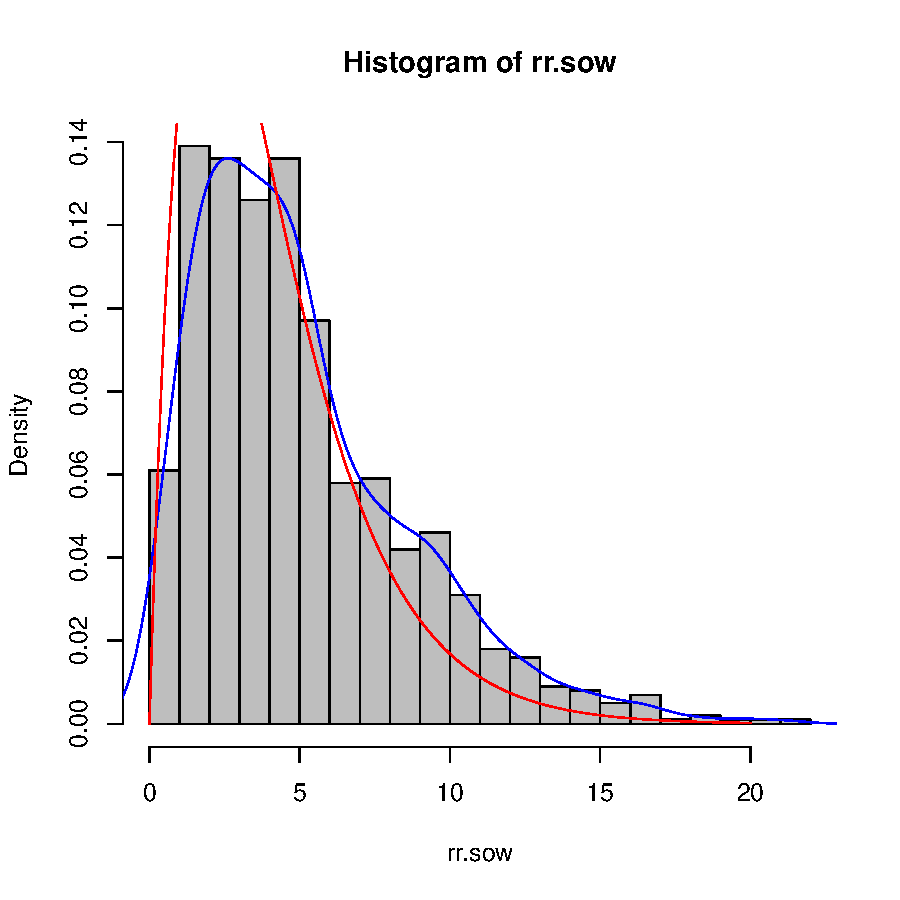
\includegraphics{figures/MMtest-011}


\begin{Schunk}
\begin{Sinput}
 xx <- seq(0,20,0.1)
 hist(rr.harv, prob=T, nclass=20, col="gray")
 lines(density(rr.harv), col="blue")
 lines(xx, dchisq(xx, df=1), col="red")
\end{Sinput}
\end{Schunk}
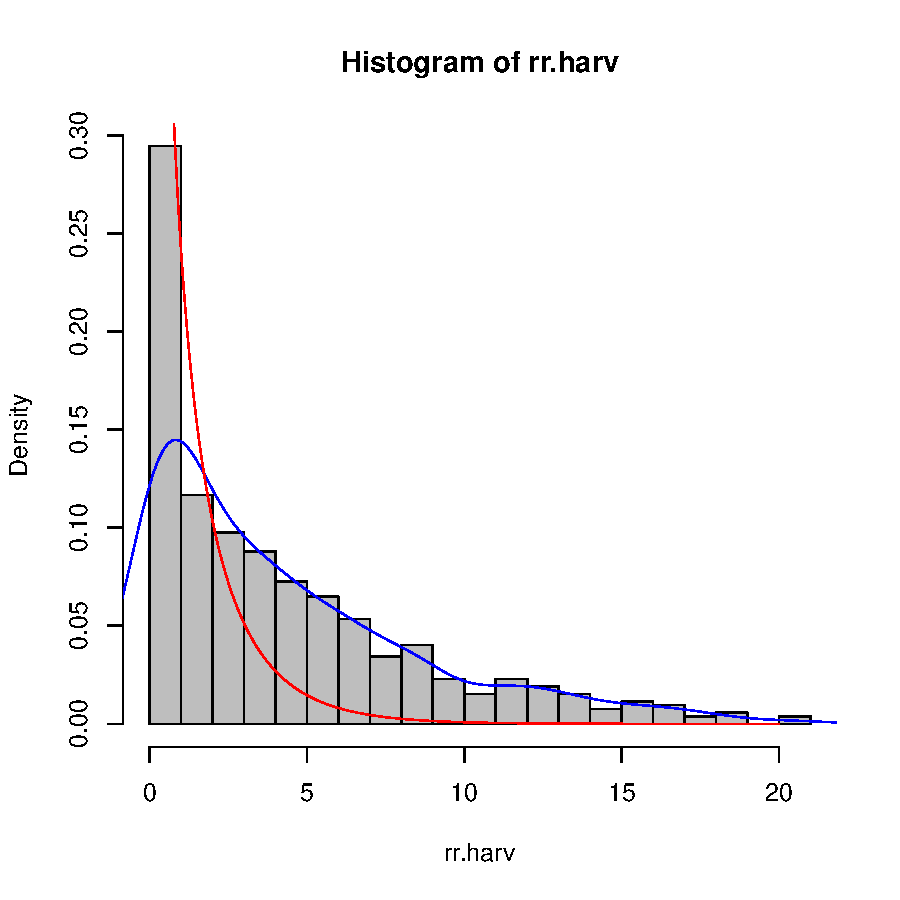
\includegraphics{figures/MMtest-012}



\subsection{Making the tests}
\label{sec:making-tests}

Tests based on a direct evaluation of tail probabilities from the
simulated reference distributions are:

\begin{Schunk}
\begin{Sinput}
 PBmodcomp(beet0, beet_no.sow, ref=rr.sow)
\end{Sinput}
\begin{Soutput}
large : sugpct ~ block + sow + harvest + (1 | block:harvest)
small : sugpct ~ block + harvest + (1 | block:harvest)
<environment: 0x07085e40>
       tobs df p
LRT    85.2  4 0
PBtest 85.2 NA 0
\end{Soutput}
\end{Schunk}

\begin{Schunk}
\begin{Sinput}
 PBmodcomp(beet0, beet_no.harv, ref=rr.harv)
\end{Sinput}
\begin{Soutput}
large : sugpct ~ block + sow + harvest + (1 | block:harvest)
small : sugpct ~ block + sow + (1 | block:harvest)
<environment: 0x06beea38>
        tobs df      p
LRT    12.91  1 0.0003
PBtest 12.91 NA 0.0574
\end{Soutput}
\end{Schunk}



Tests based on 1) making a Bartlett correction of the LRT and 2)
assuming LRT to follow a gamma distribution with mean and variance
estimated from the
simulated from the reference distribution are:



\begin{Schunk}
\begin{Sinput}
 BCmodcomp(beet0, beet_no.sow, ref=rr.sow)
\end{Sinput}
\begin{Soutput}
large : sugpct ~ block + sow + harvest + (1 | block:harvest)
small : sugpct ~ block + harvest + (1 | block:harvest)
<environment: 0x07085e40>
          tobs df p
LRT      85.20  4 0
Bartlett 67.36  4 0
Gamma    85.20 NA 0
\end{Soutput}
\end{Schunk}


\begin{Schunk}
\begin{Sinput}
 BCmodcomp(beet0, beet_no.harv, ref=rr.harv)
\end{Sinput}
\begin{Soutput}
large : sugpct ~ block + sow + harvest + (1 | block:harvest)
small : sugpct ~ block + sow + (1 | block:harvest)
<environment: 0x06beea38>
           tobs df      p
LRT      12.914  1 0.0003
Bartlett  3.052  1 0.0806
Gamma    12.914 NA 0.0499
\end{Soutput}
\end{Schunk}

In both cases we get $p$--values for the test of harvesting time which
are very close to the $p$--value from the $F$--test.


\subsection{Parallel computing of reference distribution}
\label{sec:parall-comp-refer}

We may calculate the reference distribution by parallel computing.
To do so we must do the following once (per session):

\begin{Schunk}
\begin{Sinput}
 library(snow)
 cl <- makeSOCKcluster(rep("localhost", 4))
 clusterEvalQ(cl, library(lme4))
 clusterSetupSPRNG(cl)
\end{Sinput}
\end{Schunk}

Then we can do

\begin{Schunk}
\begin{Sinput}
 rr <- PBrefdist(beet0, beet_no.harv, nsim=100, details=1, cl=cl)
\end{Sinput}
\end{Schunk}

If we use the parallel version, it is recommended to stop the cluster
BEFORE shutting down R:

\begin{Schunk}
\begin{Sinput}
 stopCluster(cl)
\end{Sinput}
\end{Schunk}

\subsection{On the usage}
\label{sec:usage}

When making the tests in Section~\ref{sec:making-tests} we used that
we had already calculated the reference distribution. It is not
necessary to calculate the reference distribution in a separate step;
we may simply do:

\begin{Schunk}
\begin{Sinput}
 PBmodcomp(beet0, beet_no.harv)
\end{Sinput}
\end{Schunk}

In this case the reference distribution will be calculated on the
fly. If we set up a cluster as described in
Section~\ref{sec:parall-comp-refer} we may speed up the computing with

\begin{Schunk}
\begin{Sinput}
 PBmodcomp(beet0, beet_no.harv,cl=cl)
\end{Sinput}
\end{Schunk}






\end{document}
